
\begin{figure}[hbt]
  \centering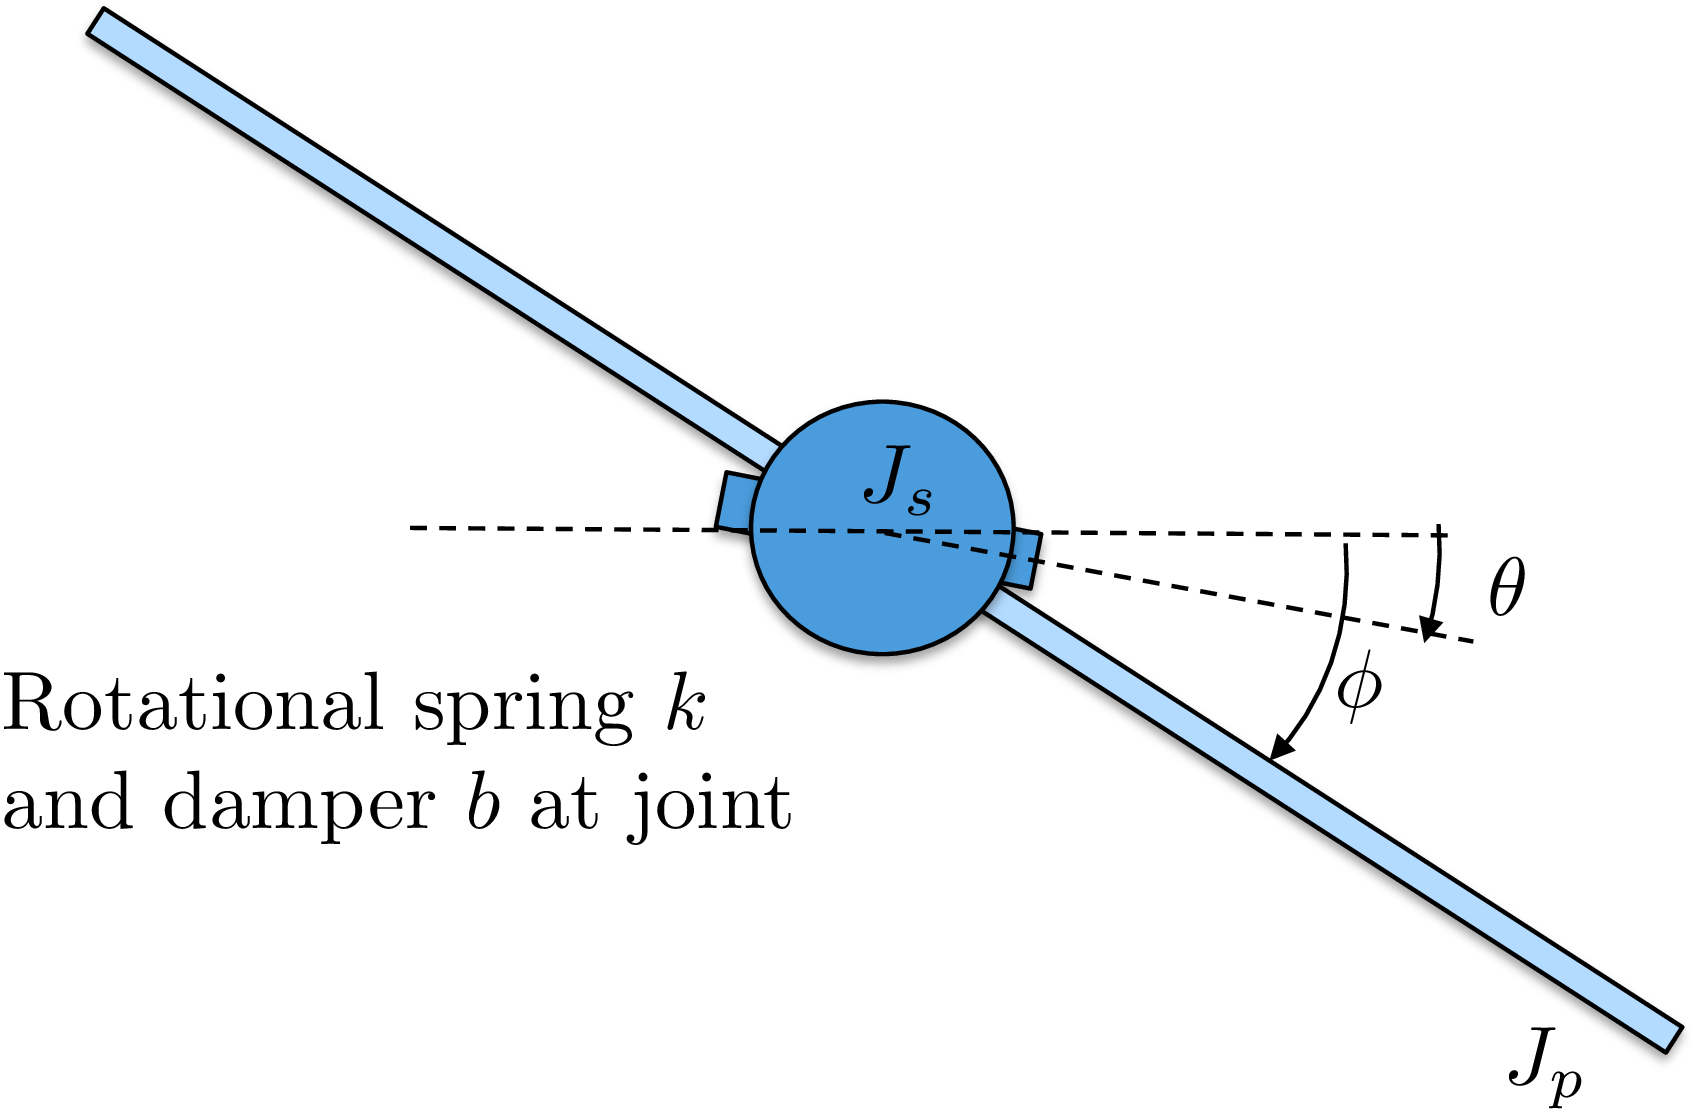
\includegraphics[width=0.5\textwidth]{6_design_studies/figures/hw_satellite_defn}
  \caption{Satellite with flexible solar panels.}
  \label{fig:sm_satellite_defn}  
\end{figure}



The generalized coordinates for the satellite attitude control problem are the angles $\theta$ and $\phi$.  Therefore, we define the generalized coordinates as $\mathbf{q}=(\theta, \phi)^\top$  We will assume the ability to apply torque on the main body ($\theta$) of the satellite, but not on the solar panel.  Therefore, the generalized force is $\boldsymbol{\tau} = (\tau, 0)^\top$.  We will model the dissipation (friction) forces as proportional to the relative motion between the main body and the solar panel.  Therefore, the damping term is given by
\[
-B\dot{\mathbf{q}} = \begin{pmatrix}-b(\dot{\theta}-\dot{\phi}) \\ -b(\dot{\phi}-\dot{\theta}) \end{pmatrix} = -\begin{pmatrix} b & -b \\ -b & b \end{pmatrix}\begin{pmatrix}\dot{\theta} \\ \dot{\phi}\end{pmatrix}.
\]

Using Equation~\eqref{eq:satellite_kinetic_energy}, the kinetic energy can be written in terms of the generalized coordinates as
\begin{align*}
K(\mathbf{q},\dot{\mathbf{q}}) &= \frac{1}{2} J_s \dot{\theta}^2 + \frac{1}{2} J_p \dot{\phi}^2 \\
&= \frac{1}{2} J_s \dot{q}_1^2 + \frac{1}{2} J_p \dot{q}_2^2.
\end{align*}
The potential energy of the system is due to the spring force between the base and the solar panel, and is given by
\begin{align*}
P(\mathbf{q}) &= \frac{1}{2} k (\phi-\theta)^2 \\
&= \frac{1}{2} k (q_2-q_1)^2,
\end{align*}
where $k$ is the spring constant. 
The Lagrangian is therefore given by
\[
L(\mathbf{q},\dot{\mathbf{q}}) = \frac{1}{2} J_s \dot{q}_1^2 + \frac{1}{2} J_p \dot{q}_2^2 - \frac{1}{2} k (q_2-q_1)^2.
\]
Therefore
\begin{align*}
\frac{\partial L}{\partial\dot{\mathbf{q}}} &= \begin{pmatrix} 
J_s\dot{\theta} \\
J_p\dot{\phi}
\end{pmatrix} \\
\frac{\partial L}{\partial\mathbf{q}} &= \begin{pmatrix}
k(\phi-\theta) \\
-k(\phi-\theta)
\end{pmatrix}.
\end{align*}
Differentiating $\frac{\partial L}{\partial \dot{\mathbf{q}}}$ with respect to time gives
\[
\frac{d}{dt}\left(\frac{\partial L}{\partial \dot{\mathbf{q}}}\right) = \begin{pmatrix} 
J_s\ddot{\theta} \\
J_p\ddot{\phi}
\end{pmatrix}.
\]
Therefore the Euler-Lagrange equation
\[
\frac{d}{dt}\left(\frac{\partial L}{\partial\dot{\mathbf{q}}} \right) - \frac{\partial L}{\partial \mathbf{q}} =  \boldsymbol{\tau} -B\dot{\mathbf{q}}
\]
gives
\[
\begin{pmatrix}
J_s\ddot{\theta} - k(\phi-\theta) \\
J_p\ddot{\phi} + k(\phi-\theta)
\end{pmatrix}
=  \begin{pmatrix} \tau \\ 0 \end{pmatrix} + \begin{pmatrix} -b(\dot{\theta}-\dot{\phi}) \\ -b(\dot{\phi}-\dot{\theta}) \end{pmatrix}.
\]
Simplifying and moving all second order derivatives to the left-hand side, and all other terms to the right-hand side gives
\[
\begin{pmatrix}
J_s\ddot{\theta} \\
J_p\ddot{\phi}
\end{pmatrix}
= \begin{pmatrix}  \tau -b(\dot{\theta}-\dot{\phi})-k(\theta-\phi) \\ -b(\dot{\phi}-\dot{\theta}) - k(\phi-\theta) \end{pmatrix}.
\]
Using matrix notation, this equation can be rearranged to isolate the second order derivatives on the left-hand side as
\begin{equation}\label{eq:satellite_sim_model}
\begin{pmatrix}
J_s & 0 \\ 
0 & J_p
\end{pmatrix} \begin{pmatrix}\ddot{\theta} \\ \ddot{\phi} \end{pmatrix}
= \begin{pmatrix} \tau-b(\dot{\theta}-\dot{\phi})-k(\theta-\phi) \\ -b(\dot{\phi}-\dot{\theta}) - k(\phi-\theta) \end{pmatrix}.
\end{equation}
Equation~\eqref{eq:satellite_sim_model} represents the simulation model for the simplified satellite system.
